\chapter{实验结果及分析、讨论}
\label{cha:re}

本章展示的实验数据,可通过调用程序相应部分复现。实验分析部分基于文献搜索结果。

\section{模块单元结果}

\subsection{图像的滤波处理}

对某相机拍摄的PNG图片,读取RGB颜色空间后,处理效果如\autoref{fig:hw1}:(其中从左上角,以先从左到右,再从上到下的顺序标数,第一张图像为原图,第二张图像为最大值取样,第三张图像为平均值取样,第四张图像为加权平均值取样(Luminance))

\begin{figure}[H]
    \centering
    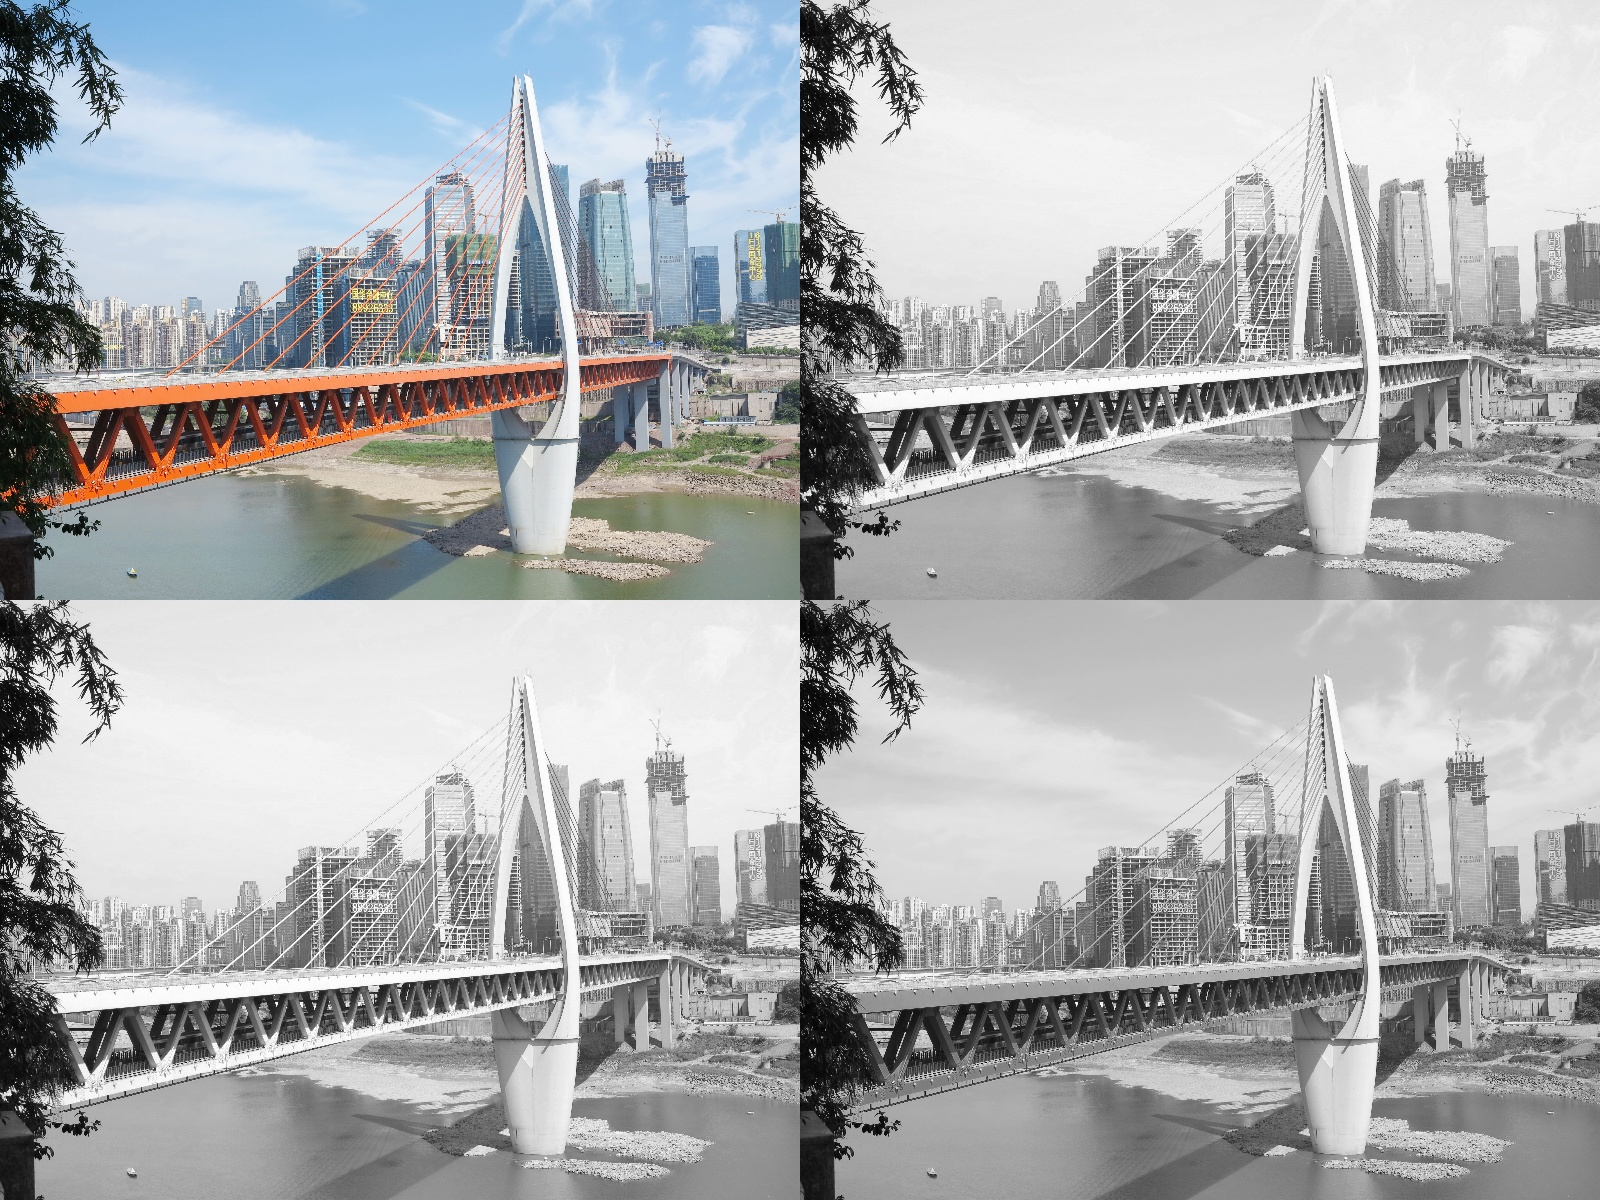
\includegraphics[width=.5\columnwidth]{hw1.jpg}
    \caption{灰度处理实验结果}
    \label{fig:hw1}
\end{figure}

根据人眼观察,在这种情况进行灰度空间转换时,使用加权平均值取样对这张图片的还原度最大,其明度较高的细节,如蓝天白云、红色桥梁等得到了充分保留。而后对数据库内人脸进行同等处理,也得到类似的直观结论。(所以电子行业用这个标准,还是有原因的!)

另外,在使用MATLAB或Python numpy库直接对读取图像进行处理时,很容易忽略数据类型的问题。对于正常的8位3通道图片,各像素点的数据均以\verb|uint8|的形式储存,在加权求和时,由于人脸数据库中图片明度普遍较高,故通道先求和,所得值将超过$2^8-1=255$,导致结果图像数据失真。可以调用平均值函数,或者数据类型转换来无损的解决这个问题。

需要注意的是,若要对这一结果进行深入研究,除了分析观察值外,还要结合其应用场景进行分析。此处,鉴于主流的图像处理工具(Matlab, OpenCV)均使用了Luminance加权平均值取样,故不再具体探讨其对实验结果的影响。为直击重点,本实验也不再探讨直方图优化、伽玛校正的原理,及其与灰度转换相结合的具体作用效果。

\begin{figure}[H]
    \centering
    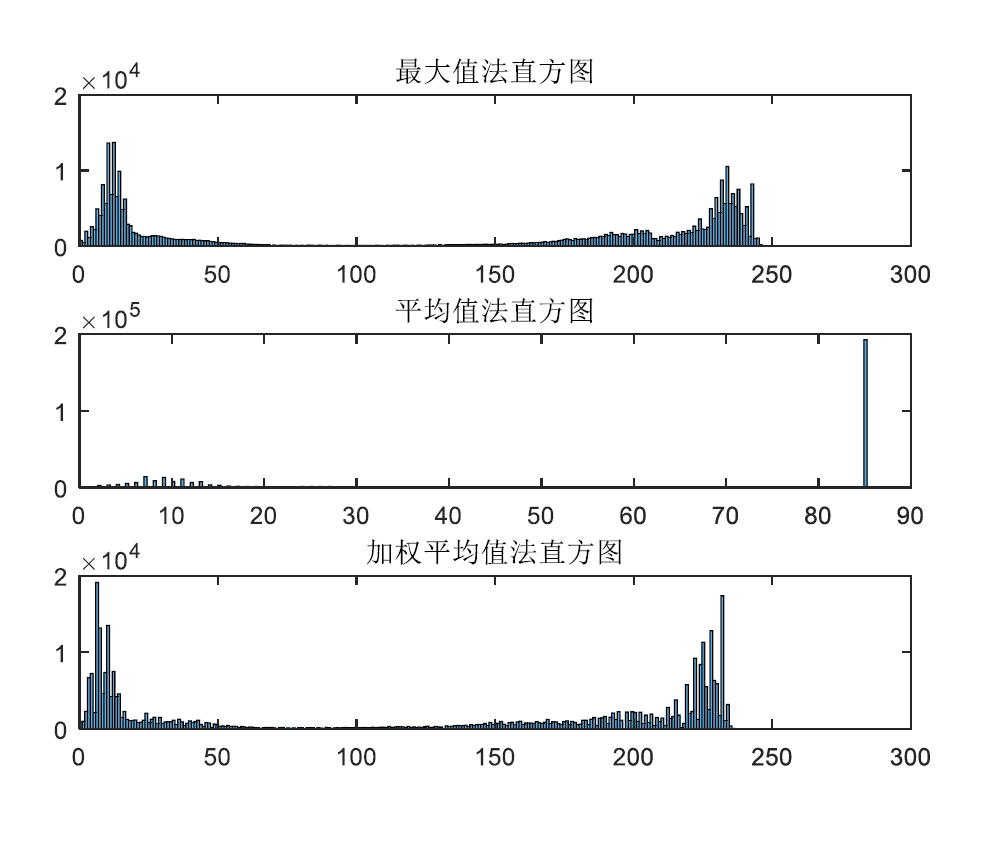
\includegraphics[width=.5\columnwidth]{hw1_add.png}
    \caption{某人脸图片经不同灰度处理后的直方图结果}
    \label{fig:hw1_add}
\end{figure}

\textbf{综上,经分析,程序主模块最终采用本部分的加权平均值取样部分(浮点输出)。}

\subsection{图像的主成分分析}

对数据库中训练库、测试库中的部分照片进行多种去噪处理,并将其图片输出,过中心的平行、垂直线上像素的R通道值的绘图数据,各像素点R通道8位值数据的直方图制作成图表,结果如下。

\begin{figure}[H]
    \centering
    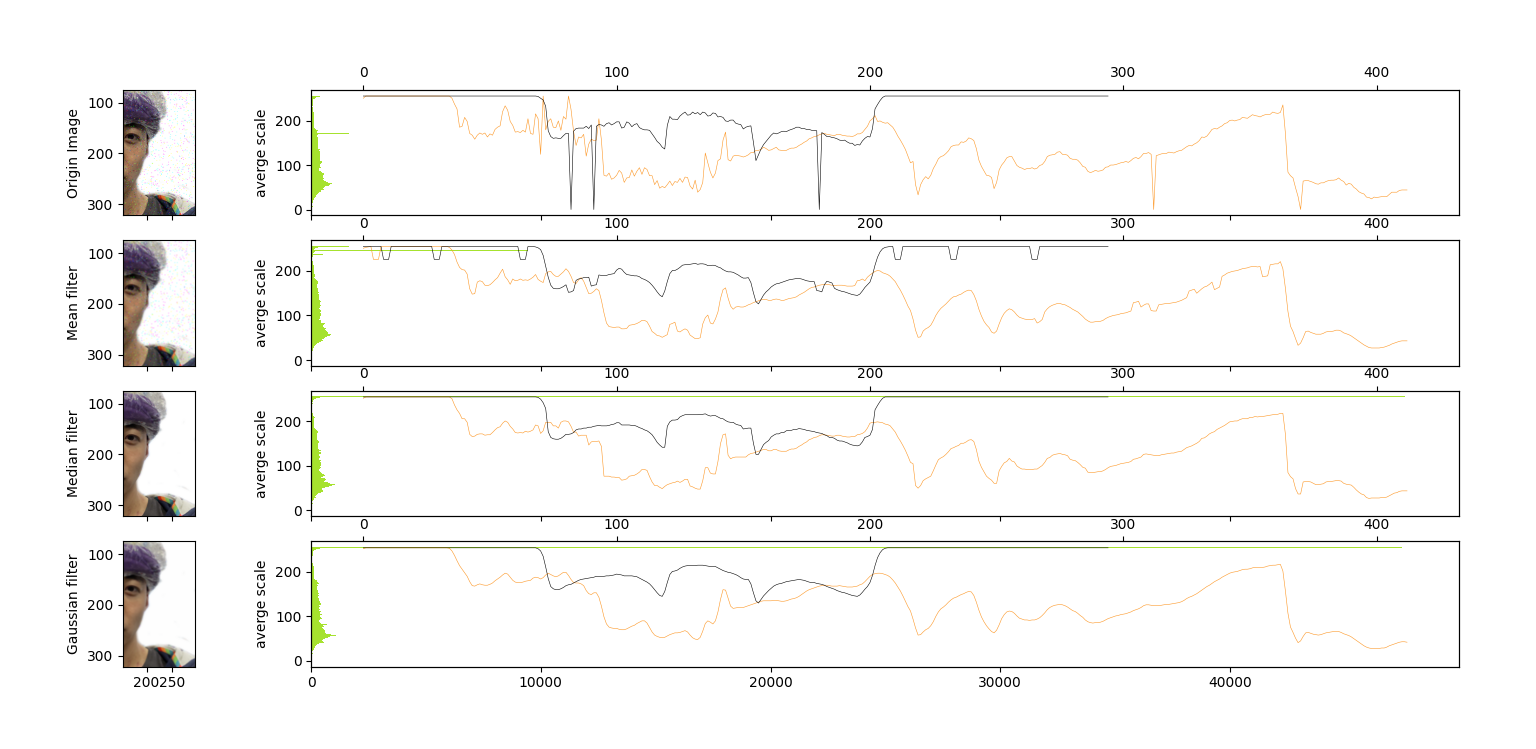
\includegraphics[width=.81\columnwidth]{hw2_fig1.png}
    \caption{三种滤波处理后的输出结果}
    \label{fig:hw2_1}
\end{figure}

\begin{figure}[H]
    \centering
    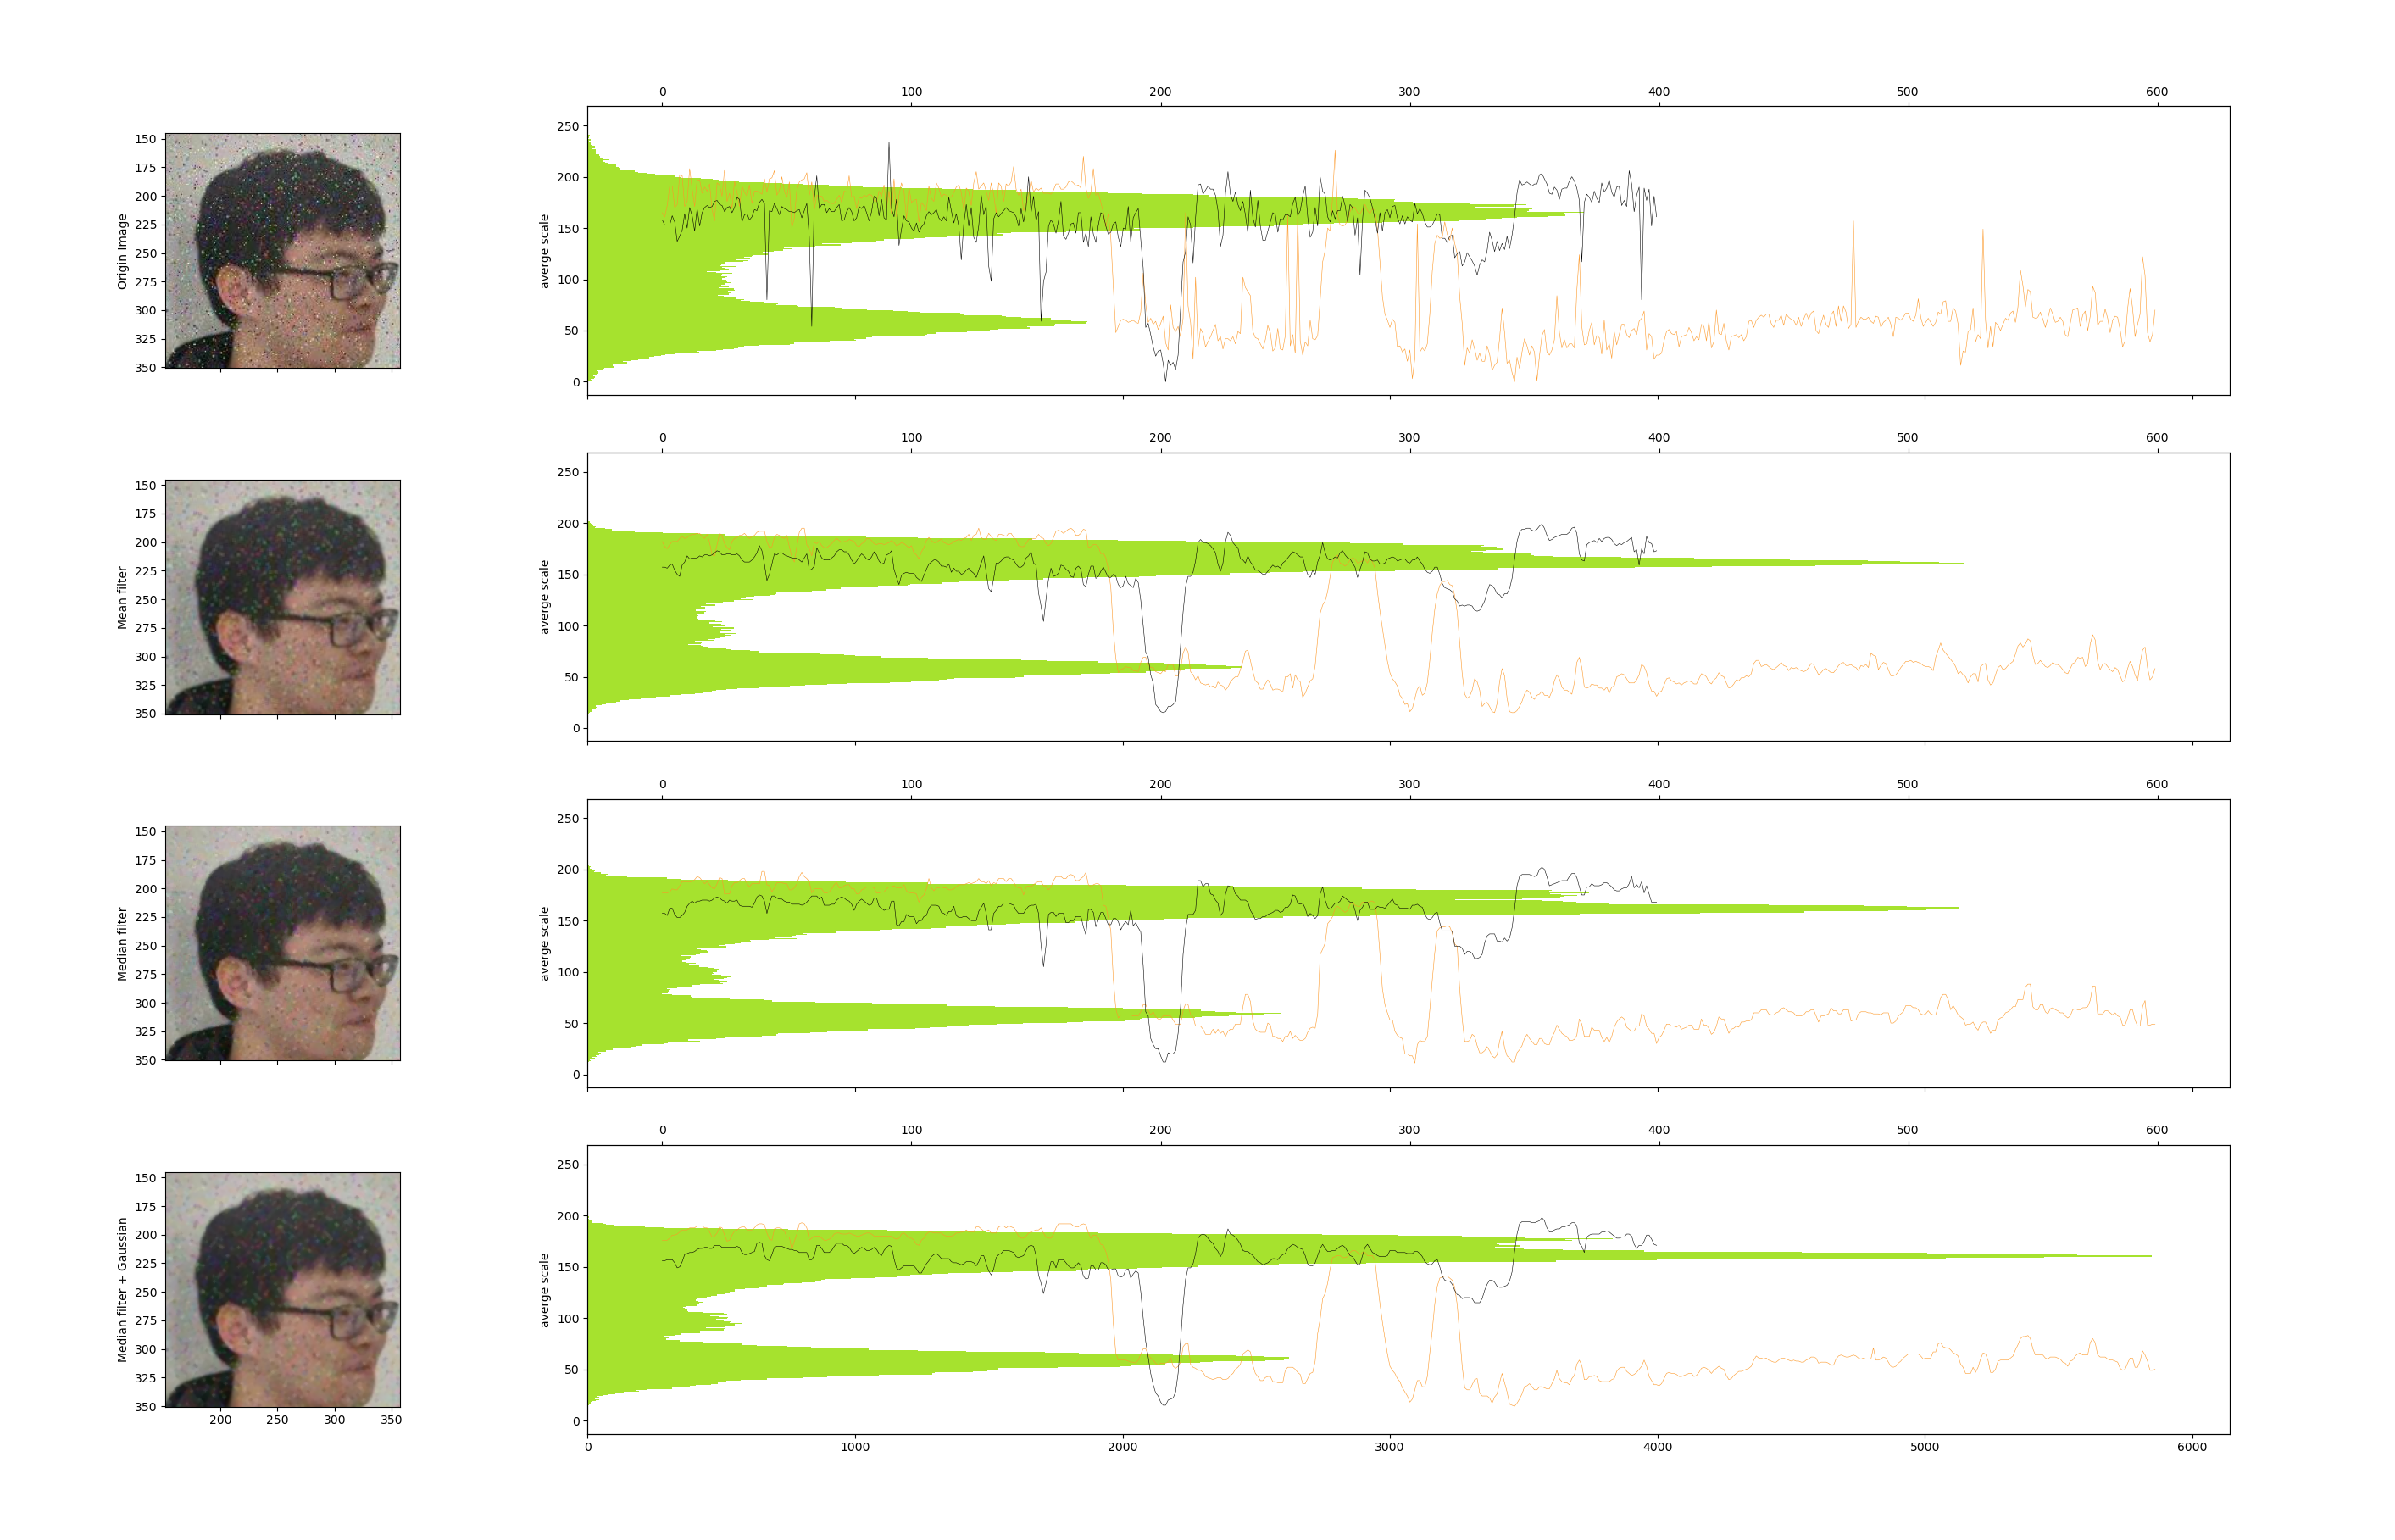
\includegraphics[width=.81\columnwidth]{hw2_fig2.png}
    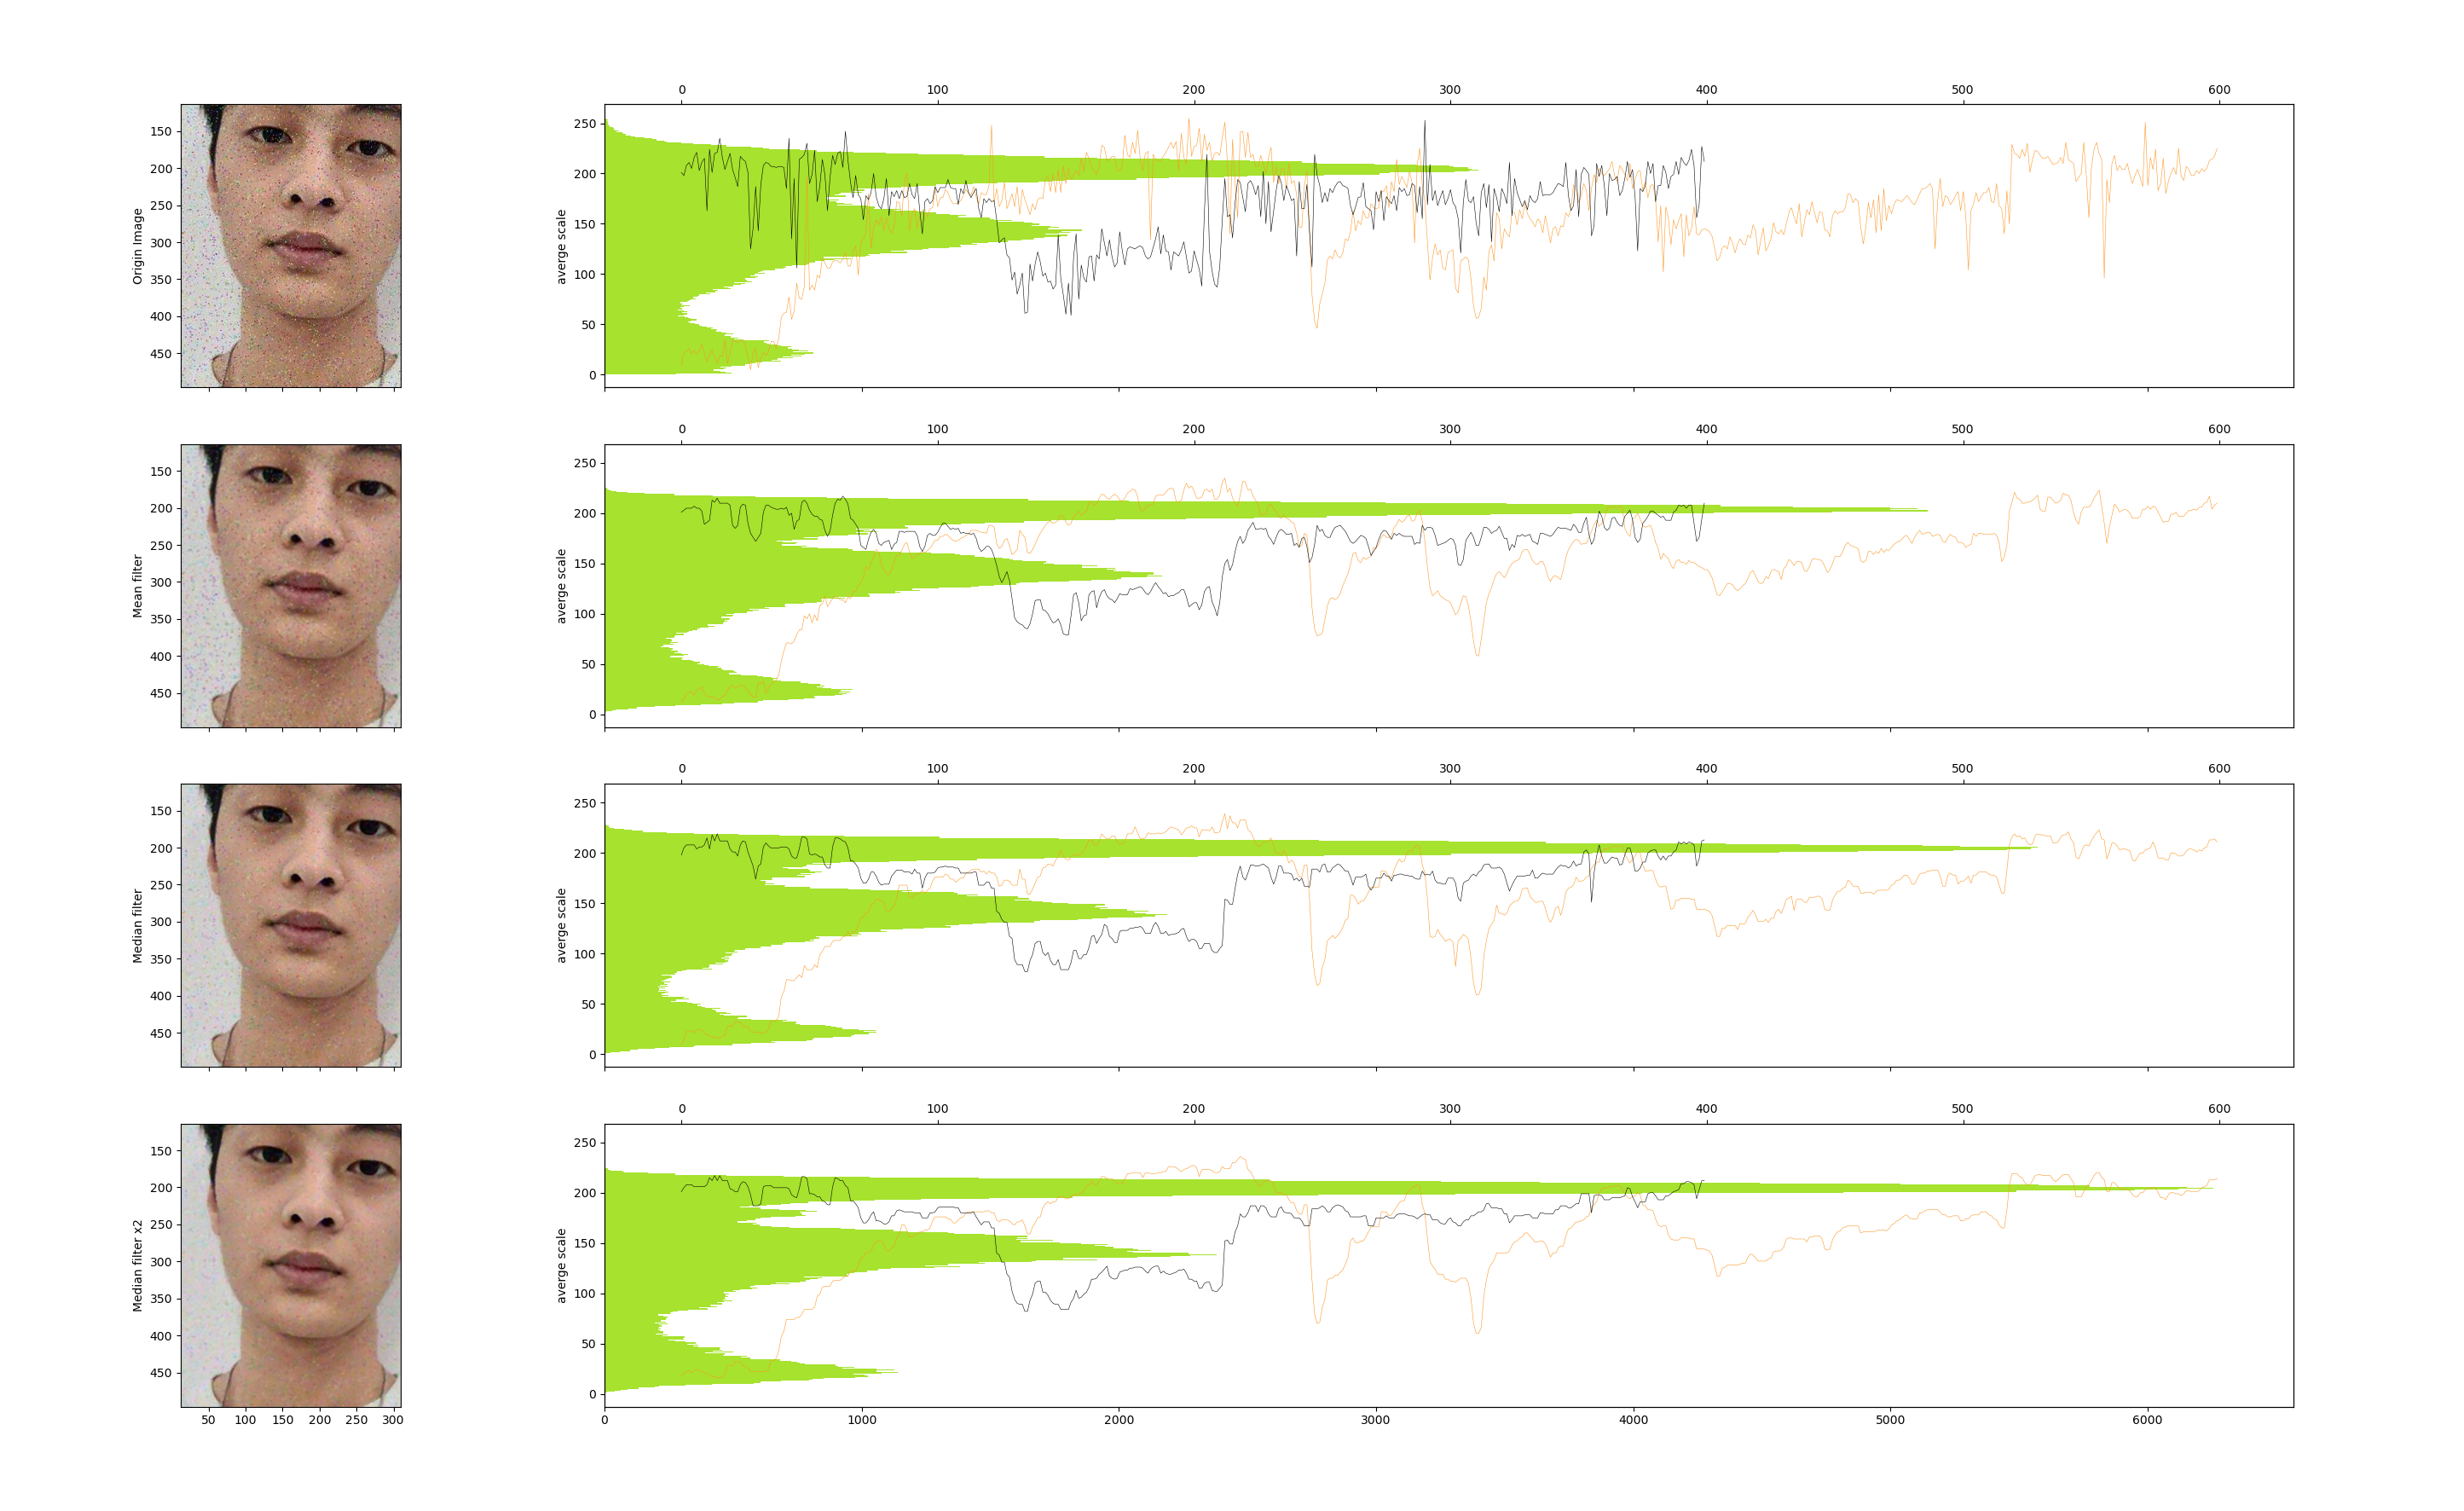
\includegraphics[width=.81\columnwidth]{hw2_fig3.png}
    \caption{分别展示了高斯滤波后中值滤波,两次中值滤波的输出结果}
    \label{fig:hw2_2}
\end{figure}

\autoref{fig:hw2_1}自上而下,展示了原图、均值滤波、中值滤波、高斯滤波的相应结果。可以发现均值滤波对椒盐噪声去除效果不好,另外两种滤波对简单的椒盐噪声去除效果较好。

\autoref{fig:hw2_2}的第一张后两行展示的分别是中值滤波、高斯滤波后中值滤波的输出结果,可以发现高斯滤波反而会增强高密度的椒盐噪声。其第二张后两行展示的分别是一次中值滤波、两次中值滤波的输出结果,可以发现二次中值滤波对噪声还有一定的削减作用。次数再次升高后,效果不再明显。

\textbf{综上,经分析,程序主模块最终采用本部分的中值滤波,并连续调用两次。}

\section{识别、交互系统结果}

\subsection{处理时间}
\label{sec:pca0}

\textbf{在本机}统计了训练模块中较为耗时的两部分:中值滤波处理和样本库主成分分析。不采用中值滤波的耗时为3.4\~4.9s,采用未加速的中值滤波耗时约为18min51s(每张图耗时约5s),numba加速的中值滤波耗时为15.5\~20.4s;主成分分析的耗时为4.2\~9.1s。

识别模块中耗时的主要部分为测试集批量读入,可同等看待。

\begin{figure}[h]
    \centering
    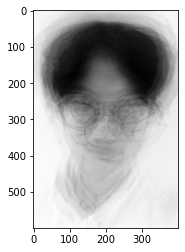
\includegraphics[width=.4\columnwidth]{eig_single.png}
    \caption{单组样本训练得到的第一个主特征,经可视化处理。}
    \label{fig:eig_single}
\end{figure}

\subsection{识别准确度}

对kNN分类算法和选取的主成分进行调整,发现当 $k=4$ 时,主成分最少仅需容纳前$12$维即可达到最佳识别正确率。仅\autoref{fig:class1}所示的样本无法被正确识别。增大主成分维数,识别结果基本不受影响。而增大 $k$ 值会导致部分测试样本匹配到其他类型的人脸。

样本12在$k$、$d$较高时才能被正常识别,如$k=27, d=185$。故样本12的训练集有过拟合的倾向。

\begin{figure}[H]
    \centering
    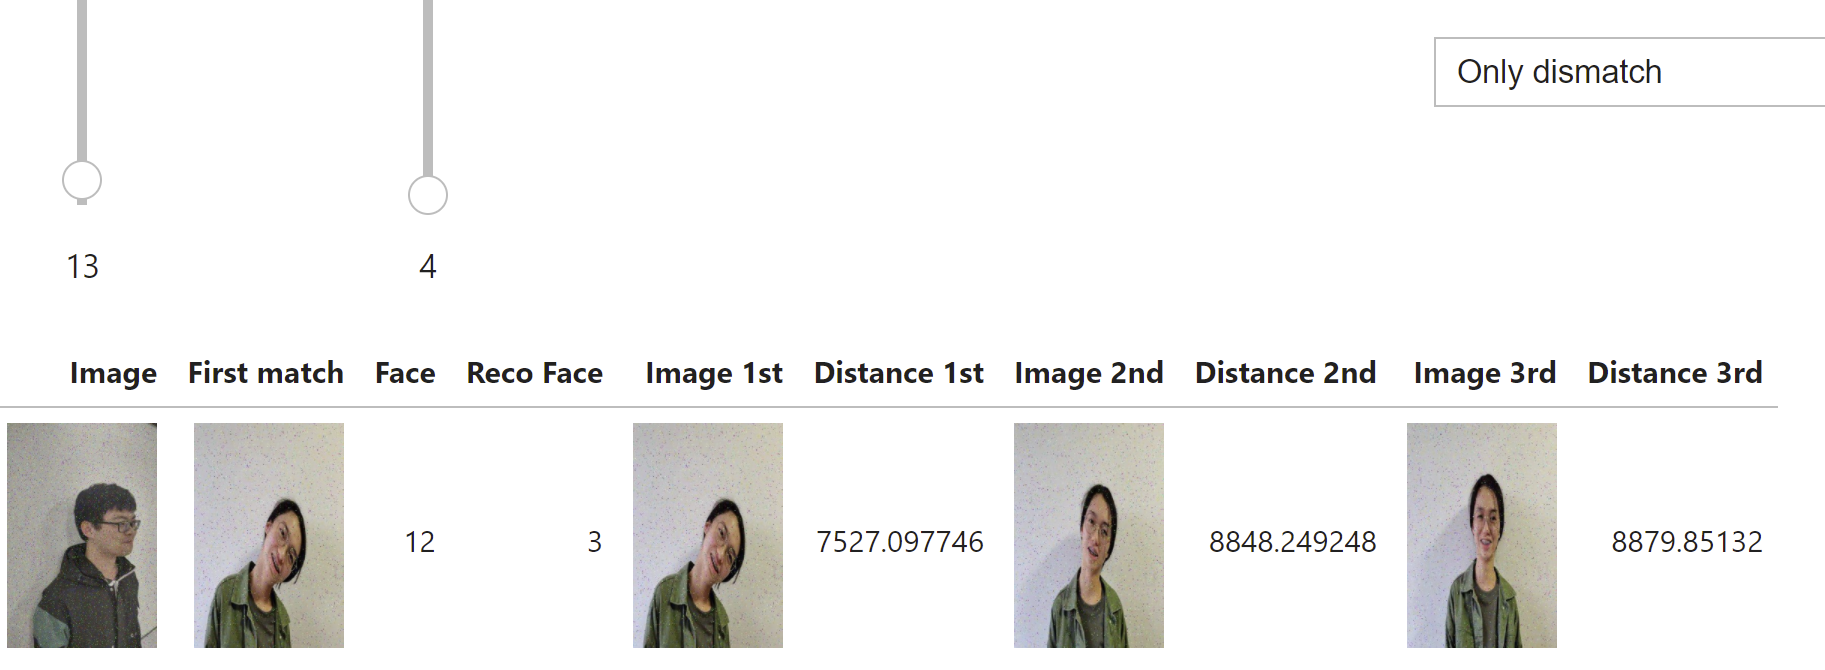
\includegraphics[width=.8\columnwidth]{class1.png}
    \caption{无法匹配的样本图片和识别输出结果}
    \label{fig:class1}
\end{figure}

\section{识别的调整及优化}

下列的数据展示了选取前$d$维主成分和$k$个临近数据集点后的分类情况。注意到有部分测试数据十分接近于训练数据,经查看文件,其中有部分测试图片与训练图片完全一样,另有一些是噪声不同。

\begin{minted}[breaklines]{xml}
d=20, k=4
test face 3 is too close to dataset(s3_1)?
test face 4 is too close to dataset(s4_3)?
test face 9 is too close to dataset(s9_1)?
12 3 [[9.92052951e+03 1.60000000e+01 3.00000000e+00]
 [9.92129420e+03 1.90000000e+01 3.00000000e+00]
 [1.06769758e+04 1.88000000e+02 2.40000000e+01]
 [1.06920015e+04 1.80000000e+01 3.00000000e+00]]
test face 22 is too close to dataset(s22_3)?
Error rate is 0.05.

d=120, k=4
test face 3 is too close to dataset(s3_1)?
7 15 [[[1.41684977e+04 5.80000000e+01 7.00000000e+00]
 [1.62357532e+04 1.23000000e+02 1.50000000e+01]
 [1.70395660e+04 1.20000000e+02 1.30000000e+01]
 [1.92705277e+04 1.22000000e+02 1.50000000e+01]]
test face 9 is too close to dataset(s9_1)?
12 3 [[1.61600607e+04 1.80000000e+01 3.00000000e+00]
 [1.71320333e+04 1.88000000e+02 2.40000000e+01]
 [1.71812421e+04 1.00000000e+01 1.00000000e+00]
 [1.78519738e+04 1.60000000e+01 3.00000000e+00]]
 test face 22 is too close to dataset(s22_3)?
Error rate is 0.1.
\end{minted}

那么我们拿完全不滤去噪声的训练集和测试集来跑跑看呢?好家伙,噪声似乎真的被当作一个特征,留存在高维度的主成分里了。只考虑低维度的主成分,噪声对分类的影响反而不大。

\begin{minted}[breaklines]{xml}
d=6, k=5
test face 1 is too close to dataset(s1_7)?
test face 3 is too close to dataset(s3_1)?
test face 9 is too close to dataset(s9_1)?
13 12 [[ 6279.65703444   175.            23.        ] [11301.58253784   102.            12.        ]]
test face 22 is too close to dataset(s22_3)?
23 5 [[ 8416.09473533   171.            23.        ] [10590.35552612   174.            23.        ]]
Error rate is 0.1.

d=100, k=5
6 3 [[1.34565528e+04 4.40000000e+01 6.00000000e+00] [1.50439833e+04 4.50000000e+01 6.00000000e+00]]
7 15 [[9.86112416e+03 5.80000000e+01 7.00000000e+00] [1.64500187e+04 1.22000000e+02 1.50000000e+01]]
8 22 [[10763.33564653   163.            22.        ] [12367.46637443   162.            22.        ]]
test face 9 is too close to dataset(s9_1)?
13 23 [[2.06595640e+04 1.75000000e+02 2.30000000e+01] [2.58334201e+04 1.70000000e+02 2.20000000e+01]]
23 5 [[2.16220804e+04 1.71000000e+02 2.30000000e+01] [2.55125896e+04 3.20000000e+01 5.00000000e+00]]
Error rate is 0.25.
\end{minted}

\subsection{生成特征向量分析}
\label{sec:eig}

将中值滤波前后的主成分分析工具:特征向量进行比较,更可以发现一些有趣的现象。

\begin{figure}[H]
    \centering
    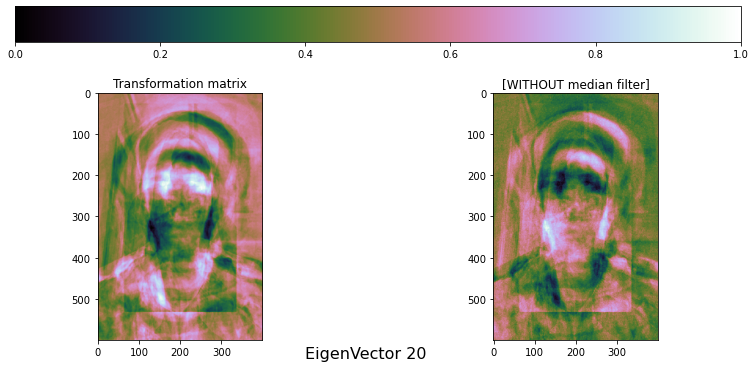
\includegraphics[width=.8\columnwidth]{eig_20.png}
    \caption{$d=20$时的特征向量输出}
    \label{fig:eig_20}
\end{figure}

颜色空间是按照百分比的方式(0~1)对归一化的特征向量进行绘制的。不同方式生成的特征向量,有时候会接近相似,有时会大相径庭,但有时候却会……完全相反?

\begin{figure}[H]
    \centering
    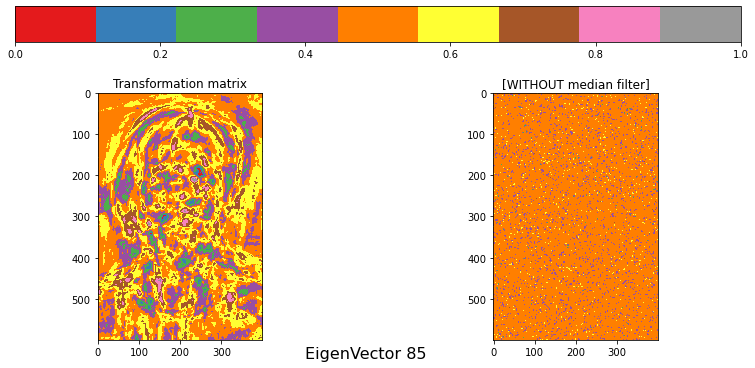
\includegraphics[width=.8\columnwidth]{eig1.png}
    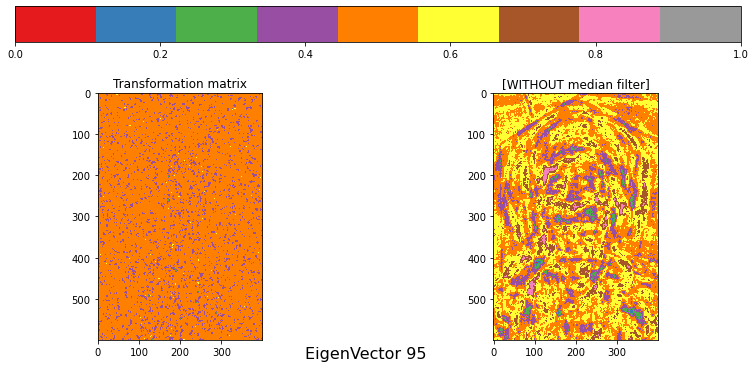
\includegraphics[width=.8\columnwidth]{eig2.png}
    \caption{$d=85$和$d=95$时的特征向量输出}
    \label{fig:eig}
\end{figure}

随着维数增大,两种特征向量里都出现了噪声形成的主成分,且中值滤波前的主成分为噪声的维数更多。这说明生成的噪声过于密集,造成了两个结果:

1.噪声重合形成了一定的规律,并被代数方法所单独识别出来。(这听上去就很无监督学习。)否则,噪声应基本在含有人脸的特征向量中显现。(实际上,两种特征向量里也都有这种情况)

2.套用的中值滤波方式仍不能很好的去除现有的噪声。

那么是时候总结一下了。